\documentclass[12pt]{article}
\usepackage{mathtools}
\usepackage{amssymb}
\usepackage{amsthm}
\usepackage{pgfplots}
\usepackage{tikz}
\usetikzlibrary{calc}
\usepackage{polski}
\usepackage[utf8]{inputenc}
\usepackage{geometry}
\usepackage{amsmath}
\usepackage{gensymb}
\usepackage{mnsymbol}
\usepackage{graphicx}
\usepackage{textgreek}
\usepackage{float}
\usepackage{caption}
\begin{document}
\newgeometry{tmargin=2cm,bmargin=2cm,lmargin=2cm,rmargin=2cm}
\tableofcontents \newpage
\section{Cel ćwiczenia}
Celem ćwiczenia było poznanie podstawowych wielkości opisujących pole elektrostatyczne oraz wyznaczenie powierzchni ekwipotencjalnych i wektorów natężenia pola elektrycznego na płaszczyźnie różnych konfiguracji elektrod.
\section{Wstęp teorytyczny}
Rozpatrzmy zamkniętą powierzchnię obejmującą dwa ładunki $Q_1$ i $Q_2$. Całkowity strumień (liczba linii sił) przechodzący przez powierzchnię otaczającą ładunki $Q_1$ i $Q_2$ jest równy: \newline \newline
{\Large $\phi_c=\oint\bold{E}d\bold{S}=\oint(\bold{E}_1+\bold{E}_2)d\bold{S}=\oint\bold{E}_1d\bold{S}+\oint\bold{E}_2d\bold{S}$}, \newline \newline
gdzie pole $E_1$ jest wytwarzane przez $Q_1$, a pole $E_2$ przez $Q_2$. Kółko na znaku całki oznacza, że powierzchnia całkowania jest zamknięta. Zachodzi wtedy: \newline \newline
{\Large $\phi_c=\frac{Q_1}{\varepsilon_0}+\frac{Q_2}{\varepsilon_0}=\frac{Q_1+Q_2}{\varepsilon_0}$} \newline \newline
Całkowity strumień pola elektrycznego przez zamkniętą powierzchnię jest więc równy całkowitemu ładunkowi otoczonemu przez tę powierzchnię podzielonemu przez $\varepsilon_0$. Analogiczne rozumowanie można przeprowadzić dla dowolnej liczby ładunków wewnątrz dowolnej zamkniętej powierzchni. Otrzymujemy więc ogólny związek znany jako prawo Gaussa: \newline \newline
{\Large $\oint\bold{E}d\bold{S}=4\pi{k}Q_{wewn.}=\frac{Q_{wewn.}}{\varepsilon_0}$} \newline \newline
Układ dwóch jednakowych co do wartości ładunków elektrycznych, mających przeciwne znaki nazywany jest dipolem elektrycznym. W przypadku dipola ładunki znajdują się na tyle blisko siebie, że pola elektrostatyczne przez nie wytworzone wpływają wzajemnie na siebie, w wyniku czego linie pola centralnego pojedynczych ładunków ulegają zakrzywieniu.\newline
\begin{figure}[H]
\centering
\includegraphics[width=7cm]{1}
\caption*{\textbf{Rys. 1}: Powierzchnie ekwipotencjalne (linie przerywane) i linie sił pola (linie ciągłe) dipola elektrycznego}
\end{figure} 
\noindent Powierzchnie ekwipotencjalne (linie przerywane) i linie sił pola (linie ciągłe) dipola elektrycznego; linie ekwipotencjalne oznaczają przecięcia powierzchni ekwipotencjalnych z płaszczyzną rysunku. 
Mówimy, że w danym obszarze istnieje jednorodne pole elektryczne, jeżeli w każdym punkcie tego obszaru wartość natężenia pola jest jednakowa.
Jednorodne pole elektryczne wytwarzamy na przykład między okładkami kondensatora płaskiego.\newline
Kondensator płaski tworzą dwie równoległe naładowane płyty metalowe (każda z płyt ma ładunek przeciwny do drugiej). Linie sił pola jednorodnego są wzajemnie równoległe.
W jednorodnym polu elektrycznym zależność między natężeniem pola elektrycznego a różnicą potencjałów wyraża się wzorami:
{\Large $E=\frac{\Delta{V}}{d}$            lub           $E=\frac{U}{d}$}
gdzie $\Delta{V}$ to różnica potencjałów płyt kondensatora (inaczej napięcie $U$), zaś $d$ to odległość płyt kondensatora. \newline
Przybliżoną wartość natężenia pola $E$ możemy uzyskać obliczając numerycznie gradient potencjału: \newline \newline
{\Large $E_x=-\frac{\partial{V}}{\partial{x}}\approx\frac{V(x+h,y)-V(x,y)}{h}$ \newline \newline
$ E_y=-\frac{\partial{V}}{\partial{y}}\approx\frac{V(x,y+k)-V(x,y)}{k}$}, \newline \newline
gdzie $h$ i $k$ są krokami siatki. \newline  
Wewnątrz kondensatora płaskiego pole elektryczne jest jednorodne, o wartości: \newline \newline
{\Large $E=\frac{U}{d}$} \newline \newline
Potencjał rośnie liniowo od zera do wartości napięcia zasilacza $U$: \newline \newline
{\Large $V(x)=\frac{U}{d}x$} \newline \newline
Na zewnątrz kondensatora płaskiego pole jest niejednorodne oraz rozproszone. \newline
Wewnątrz kondensatora cylindrycznego natężenie pola elektrycznego jest dane wzoremi: \newline \newline
{\Large$E(x)=\frac{U}{x*ln(\frac{r_z}{r_w})}$} \newline \newline
Poprzez obliczenie pochodnej z wzoru $E(x)$ otrzymujemy wyrażenie na potencjał: \newline \newline
{\Large $V(x)=\frac{U}{ln(\frac{r_z}{r_w})}ln(\frac{x}{r_z})$} \newline \newline
\newpage \section{Układ pomiarowy}
Przyrządy potrzebne do wykonania doświadczenia (Rys. 2): \newline
1. Płyty modelowe będące modelami kondensatorów: płaskiego, cylindrycznego oraz o dowolnym kształcie elektrod. \newline 
2. Zasilacz $10V$ \newline
3. Woltomierz cyfrowy \newline
\begin{figure}[H]
\centering
\includegraphics[width=14cm]{2}
\caption*{\textbf{Rys. 2}: Schemat połączeń układu pomiarowego do modelowania pola elektrycznego }
\end{figure} 
\section{Przebieg ćwiczenia}
Na początku połączyliśmy obwód elektryczny tak jak na Rys. 2 używając płyty modelowej dla kondensatora płaskiego oraz sprawdziliśmy czy napięcie zasilacza wynosi $10\;V$. Przy pomocy sondy upewniliśmy się, że dobrze podłączyliśmy płytę modelową. Następnie zmierzyliśmy wartości potencjału wzdłuż trzech różnych kierunków wewnątrz kondensatora oraz wartości $51$ punktów na zewnątrz kondensatora (Prostokąt 3$\times$17). Po wykonaniu tego podłączyliśmy płytę modelową dla kondensatora cylindryczengo oraz zmierzyliśmy wyniki wzdłuż trzech promieni. Wszystkie wyniki zapisaliśmy. \newpage
\section{Wyniki pomiarów}
\begin{figure}[H]
\centering
\includegraphics[width=9cm]{3}
\caption*{\textbf{Rys. 3}: Płaski układ elektrod z zaznaczonymi punktami pomiarów. Odległość między punktami jest równa $5\;mm$.
 Na rysunku narysowano również linie ekwipotencjalne zielonym kolorem \newline ($1.5\;V$, $3\;V$, $4.5\;V$, $6\;V$, $7.5\;V$, $9\;V$)}
\end{figure} 
\begin{figure}[H]
\centering
\includegraphics[width=14cm]{4}
\caption*{\textbf{Tab. 1}: Wyniki pomiarów potencjału dla kondensatora płaskiego na zewnątrz kondensatora.\newline Wyniki podane w takiej samej kolejności jak na rysunku.}
\end{figure} 
\begin{figure}[H]
\centering
\includegraphics[width=14cm]{5}
\caption*{\noindent\textbf{Tab. 2}: Wyniki pomiarów potencjału dla kondensatora płaskiego wewnątrz kondensatora. }
\end{figure} \newpage
\begin{figure}[H]
\centering
\includegraphics[width=17cm]{6}
\caption*{\textbf{Rys. 4}: Cylindryczny układ elektrod z zaznaczonymi punktami pomiarów. Odległość między punktami jest równa w przybliżeniu
$7-8\;mm$. Na rysunku narysowano również linie ekwipotencjalne czarnym kolorem ($6\;V$, $5\;V$, $4\;V$, $3\;V$, $2\;V$, $1\;V$) }
\end{figure} 
\begin{figure}[H]
\centering
\includegraphics[width=19cm]{7}
\caption*{\textbf{Tab. 3}: Wyniki pomiarów potencjału dla kondensatora cylindrycznego.}
\end{figure} \newpage
\section{Opracowanie wyników pomiarowych dla kondensatora płaskiego}
\subsection{Obliczenie średnich wartości potencjałów oraz wartości doświadczalnych natężenia pola}
Dla obszaru wewnątrz kondensatora obliczyliśmy średnie wartości potencjału jako średnią arytmetyczną trzech zmierzonych wartości potencjału. Dla przykładu, dla $x=5\;mm$: \newline \newline
{\Large $V_{dosw}=\frac{V_a+V_b+V_c}{3}=\frac{1.124\;V+1.144\;V+0.982\;V}{3}=1.083\;V$} \newline \newline
Pozostałe wyniki, obliczone w identyczny sposób, wpisaliśmy do Tab. 4. \newline 
Następnie obliczyliśmy wartości doświadczalne natężenia pola korzystając ze wzoru: \newline \newline
{\Large $E_{dosw}=\frac{V_{n+1}-V_n}{x_{n+1}-x_n}$} \newline \newline
Dla $x_1=5\;mm$, $x_2=10\;mm$, $V_1=1.083\;V$ oraz $V_2=2.026\;V$: \newline \newline
{\Large $x^*=\frac{x_{n+1}+x_n}{2}=\frac{10\;mm+5\;mm}{2}=7.5\;mm$ \newline \newline
$E_{dosw}=\frac{V_{n+1}-V_n}{x_{n+1}-x_n}=\frac{2.026\;V-1.083\;V}{10\;mm-5\;mm}=188.6\;\frac{V}{m}$} \newline \newline
Pozostałe wyniki, obliczone w identyczny sposób, wpisaliiśmy do Tab. 4. \newline
Na końcu policzyliśmy wartości teorytyczne używając wzorów: \newline \newline
{\Large $V_{teor}=\frac{U}{d}x$       oraz       $E_{teor}=\frac{U}{d}$} \newline \newline
Dla powyższych przykładów: \newline \newline
{\Large $V_{teor}=\frac{U}{d}x=\frac{10\;V}{50\;mm}*5\;mm=1\;V$ \newline \newline
$ E_{teor}=\frac{U}{d}=\frac{10\;V}{50\;mm}=200\;\frac{V}{m}$} \newline \newline
Wszystkie wyniki teorytyczne, obliczone w identyczny sposób, wpisaliśmy do Tab. 4.
\subsection{Wykresy zależności potencjału $V$ i natężenia pola elektrycznego $E$ od odległości $x$}
\begin{center}
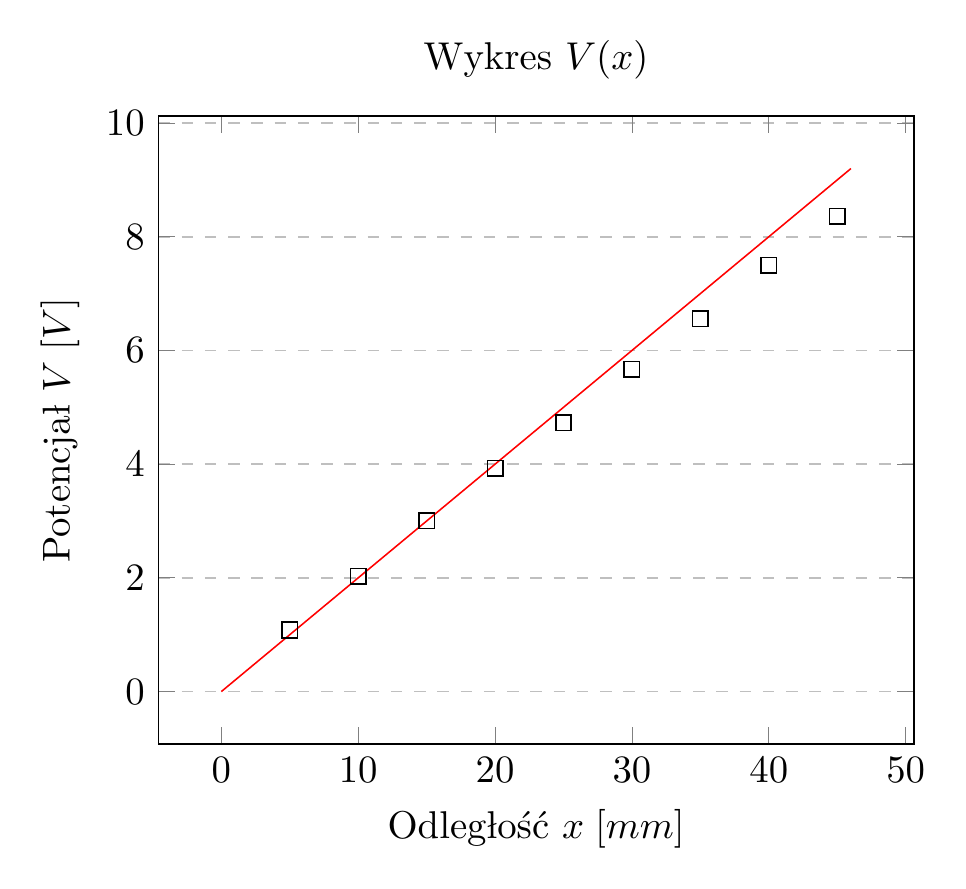
\begin{tikzpicture}[scale=1.4]
\begin{axis}[
title={Wykres $V(x)$},
xlabel={Odległość $x\;[mm]$},
ylabel={Potencjał $V\;[V]$},
legend pos=north west,
ymajorgrids=true,grid style=dashed
]

\addplot[color=black,mark=square, only marks]
coordinates {
(5,1.083)
(10,2.026)
(15,3.004)
(20,3.930)
(25,4.727)
(30,5.667)
(35,6.559)
(40,7.502)
(45,8.363)
};

\addplot [
	domain=0:46,
	samples=100,
	color=red,
] 
{0.2*x};
\end{axis}
\end{tikzpicture}
\end{center}
\begin{center}
\begin{tikzpicture}[scale=1.4]
\begin{axis}[
title={Wykres $E(x)$},
xlabel={Odległość $x\;[mm]$},
ylabel={Natężenie pola elektrycznego $E\;[\frac{V}{m}]$},
legend pos=north west,
ymajorgrids=true,grid style=dashed
]

\addplot[color=black,mark=square, only marks]
coordinates {
(7.5,188.6)
(12.5,195.6)
(17.5,185.2)
(22.5,159.4)
(27.5,188)
(32.5,178.4)
(37.5,188.6)
(42.5,172.2)
};

\addplot [
	domain=5:45,
	samples=100,
	color=red,
] 
{200};
\end{axis}
\end{tikzpicture}
\end{center}
\newpage
\subsection{Obszar na zewnątrz kondensatora}
Wartość składowych wektora $E$ można obliczyć korzystając ze wzorów: \newline \newline
{\Large $E_x=\frac{V(x+h,y)-V(x,y)}{h}$ oraz $E_y=\frac{V(x,y+k)-V(x,y)}{k}$}, \newline \newline
gdzie $h$ i $k$ są krokami siatki. U nas $h=k=5\;mm$. Dla ostatniego punktu w pierwszym wierszu Tab. 1: \newline \newline
{\Large $V(0,0)=8.439\;V$,  $V(5,0)=8.723\;V$,  $V(0,5)=8.492\;V$ \newline \newline
$E_x=\frac{8.723\;V-8.439\;V}{5\;mm}=56.8\;\frac{V}{m}$ \newline \newline
$E_y=\frac{8.492\;V-8.439\;V}{5\;mm}=10.6\;\frac{V}{m}$} \newline \newline
Obliczenia powtórzono dla kilku innych punktów oraz zaznaczono wektor natężenia pola wraz ze składowymi  na Rys. 3.
\subsection{Linie ekwipotencjalne oraz linie pola}
Linie ekwipotencjalne oraz linie pola zostały pokazane na Rys. 3.
\begin{figure}[H]
\centering
\includegraphics[width=18cm]{8}
\caption*{\textbf{Tab. 4}: Wyniki obliczeń dla kondensatora płaskiego}
\end{figure} \newpage
\section{Opracowanie wyników pomiarowych dla kondensatora cylindrycznego}
\subsection{Obliczenie średnich wartości potencjałów oraz wartości doświadczalnych natężenia pola}
Dla obszaru wewnątrz kondensatora obliczyliśmy średnie wartości potencjału jako średnią arytmetyczną trzech zmierzonych wartości potencjału. Dla przykładu, dla $x=35\;mm$: \newline \newline
{\Large $V_{dosw}=\frac{V_a+V_b+V_c}{3}=\frac{6.482\;V+6.514\;V+6.664\;V}{3}=6.533\;V$} \newline \newline
Pozostałe wyniki, obliczone w identyczny sposób, wpisaliśmy do Tab. 5. \newline 
Następnie obliczyliśmy wartości doświadczalne natężenia pola korzystając ze wzoru: \newline \newline
{\Large $E_{dosw}=\frac{V_{n+1}-V_n}{x_{n+1}-x_n}$} \newline \newline
Dla $x_1=35\;mm$, $x_2=44\;mm$, $V_1=6.533\;V$ oraz $V_2=5.047\;V$: \newline \newline
{\Large $x^*=\frac{x_{n+1}+x_n}{2}=\frac{35\;mm+44\;mm}{2}=39.5\;mm$ \newline \newline
$E_{dosw}=\frac{V_{n+1}-V_n}{x_{n+1}-x_n}=\frac{5.047\;V-6.533\;V}{44\;mm-35\;mm}=-165.11\;\frac{V}{m}$} \newline \newline
Pozostałe wyniki, obliczone w identyczny sposób, wpisaliiśmy do Tab. 5. \newline
Na końcu policzyliśmy wartości teorytyczne używając wzorów: \newline \newline
{\Large $V_{teor}=\frac{U}{ln(\frac{r_z}{r_w})}ln(\frac{x}{r_z})$       oraz       $E_{teor}=-\frac{U}{xln(\frac{r_z}{r_w})}$} \newline \newline
Dla powyższych przykładów oraz $r_w=21\;mm$,$r_z=91\;mm$: \newline \newline
{\Large $V_{teor}=\frac{U}{ln(\frac{r_z}{r_w})}ln(\frac{x}{r_z})=\frac{10\;V}{ln(\frac{91\;mm}{21\;mm})}ln(\frac{35\;mm}{91\;mm})=-6.516\;V$ \newline \newline
$ E_{teor}=-\frac{U}{xln(\frac{r_z}{r_w})}=-\frac{10\;V}{35\;mm*ln(\frac{91\;mm}{21\;mm})}=-178.31\;\frac{V}{m}$} \newline \newline
Wszystkie wyniki teorytyczne, obliczone w identyczny sposób, wpisaliśmy do Tab. 5. Ponieważ wzór użyty do obliczenia $V_{teor}$ jest innego punktu odniesienia, niż ten który był mierzony w doświadczeniu, w Tab.6 podaliśmy wartość przeciwną $V_{teor}$.

\newpage
\subsection{Wykresy zależności potencjału $V$ i natężenia pola elektrycznego $E$ od odległości $x$}
\begin{center}
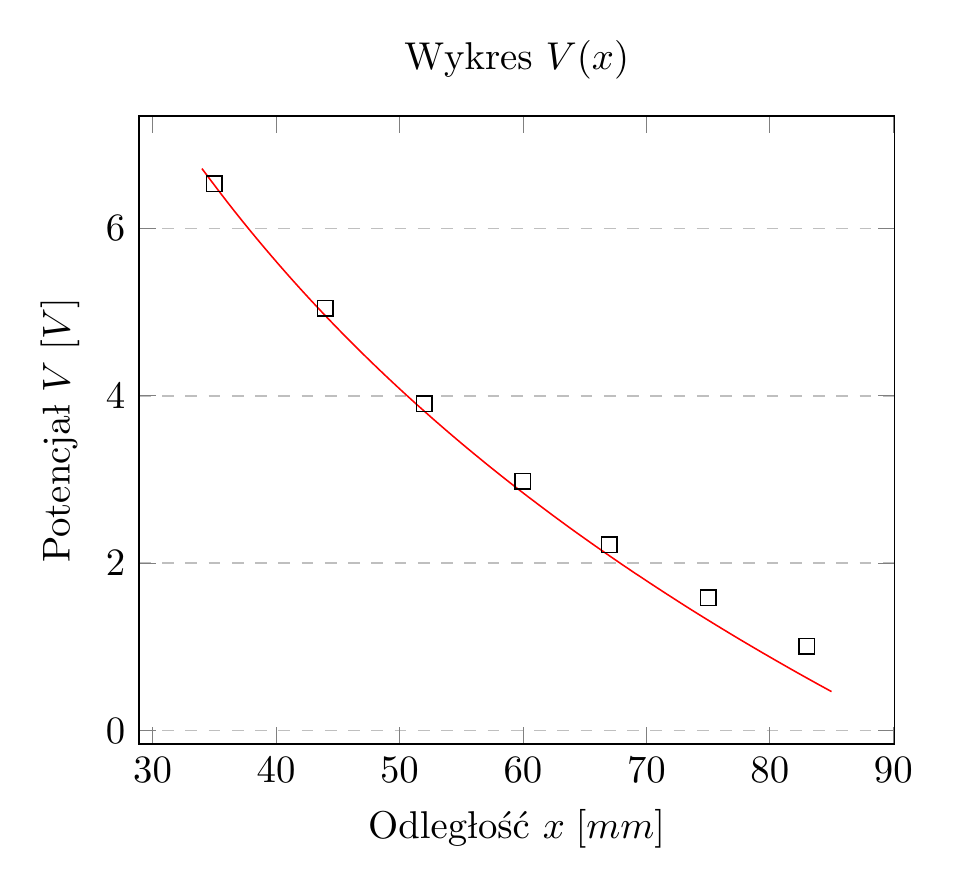
\begin{tikzpicture}[scale=1.4]
\begin{axis}[
title={Wykres $V(x)$},
xlabel={Odległość $x\;[mm]$},
ylabel={Potencjał $V\;[V]$},
legend pos=north west,
ymajorgrids=true,grid style=dashed
]

\addplot[color=black,mark=square, only marks]
coordinates {
(35,6.533)
(44,5.047)
(52,3.904)
(60,2.977)
(67,2.220)
(75,1.589)
(83,1.005)
};

\addplot [
	domain=34:85,
	samples=100,
	color=red,
] 
{(-1)*(6.81971438*ln(x/91)};
\end{axis}
\end{tikzpicture}
\end{center}
\begin{center}
\begin{tikzpicture}[scale=1.4]
\begin{axis}[
title={Wykres $E(x)$},
xlabel={Odległość $x\;[mm]$},
ylabel={Natężenie pola elektrycznego $E\;[\frac{V}{m}]$},
legend pos=north west,
ymajorgrids=true,grid style=dashed
]

\addplot[color=black,mark=square, only marks]
coordinates {
(39.5,-165.11)
(48,-142.88)
(56,-115.88)
(63.5,-108.14)
(71,-78.88)
(79,-73)
};

\addplot [
	domain=38:90,
	samples=100,
	color=red,
] 
{-1000*6.81971438/x};
\end{axis}
\end{tikzpicture}
\end{center} 
\subsection{Linie ekwipotencjalne oraz linie pola}
Linie ekwipotencjalne oraz linie pola zostały pokazane na Rys. 4.
\begin{figure}[H]
\centering
\includegraphics[width=18cm]{9}
\caption*{\textbf{Tab. 5}: Wyniki obliczeń dla kondensatora płaskiego}
\end{figure} 
\section{Wnioski}
Uzyskane wyniki dla kondensatora płaskiego okazały się nie do końca zgodne z wartościami teorytycznymi. Wewnątrz kondensatora nie wszystkie punkty pomiaru pokryły się z linią teorytyczną wyznaczoną przez wzór $V=\frac{U}{d}x$. Na zewnątrz zaś wyniki czasami malały, zamiast rosnąć. Wykres natężenia pola elektrycznego od położenia $E(x)$ nie jest linią stałą, a wszystkie obliczone punkty znajdują się pod lnią teorytyczną $E=\frac{U}{d}$. Wyniki dla kondensatora cylindrycznego okazały się bardziej zgodne, ale mimo tego nadal odbiegały od teorytycznych. Prawie wszystkie punkty pokryły się z linią teorytyczną wyznaczoną przez wzór $V=\frac{U}{ln(\frac{r_z}{r_w})}ln(\frac{x}{r_z})$. Gorzej wypadł wykres natężenia pola elektrycznego w zależności od położenia $E(x)$, w którym jedynie dwa punkty pokryły się z linią teorytyczną $E=-\frac{U}{x*ln(\frac{r_z}{r_w})}$. Niezgodności te mogą być spowodowane uszkodzeniami płyt modelowych (możliwe uszkodzenia przy zbyt mocnym nacisku sondy), zbyt małą dokładnością pomiarów przy użyciu sondy (za słabe/mocne dociśnięcie sondy) oraz niedokładności woltomierza.  
\end{document}
